\documentclass[xcolor=dvipsnames]{beamer}
\usepackage{graphicx} 
\usepackage{booktabs} 
\mode<presentation>{
    
\definecolor{MSUgreen}{RGB}{0,100,11} 
\usetheme{Boadilla}
\usecolortheme{spruce}
\setbeamercolor{block title}{bg=MSUgreen!10, fg=MSUgreen!60!black}
\setbeamercolor{navigation symbols dimmed}{fg=MSUgreen!40!white}
\setbeamercolor{navigation symbols}{fg=MSUgreen!40!white}
\setbeamertemplate{itemize item}{\color{MSUgreen}\textbullet}
\setbeamercolor{section in toc}{fg=MSUgreen}
\setbeamercolor{section number projected}{bg=MSUgreen,fg=white}
\setbeamercolor{subsection in toc}{fg=MSUgreen}
\setbeamercolor{subsection number projected}{bg=MSUgreen,fg=white}
}

\graphicspath{ {.././image/} }

\title[Machine Learning]{STRUMENTI DI ORCHESTRAZIONE E ANALISI DI WORKFLOW NEL MACHINE LEARNING}
\subtitle[]{Analisi Case Study e illustrazione Framework di Orchestrazione di pipeline di lavoro}
\author{Simone Boldrini}
\date{13 Ottobre 2021}
\institute[]{Alma Mater Studiorum - Universitá di Bologna \\ Facoltá di Scienze}

\begin{document}

\begin{frame}
    \titlepage
\end{frame}


\section*{Introduzione}
\begin{frame}
    \frametitle{Introduzione}
    
    \newtheorem{Apprendimento Automatico}{Apprendimento Automatico}

    \begin{Apprendimento Automatico}
        L'\alert{apprendimento automatico} é un ramo dell'Intelligenza Artificiale, che raccoglie metodi in grado di migliorare la performance di un algoritmo, autonomamente, nell'identificare pattern di dati.
    \end{Apprendimento Automatico}
    Gli algoritmi li suddividiamo in 3 categorie:
    \begin{itemize}
        \item Supervised Learning
        \item Unsupervised Learning
        \item Reinforcement Learning
    \end{itemize}
\end{frame}
\begin{frame}
 \frametitle{Modelli} 
 \newtheorem{Modello}{Modello}
 \begin{Modello}
Un Modello di ML é l'output generato in seguito all'addestramento dell'algoritmo.
 \end{Modello}  
 I modelli di ML assimilano i dati di training, con l'obiettivo di individuare potenziali relazioni tra i dati di input e quelli di output.
\end{frame}



    \begin{frame}
    \setbeamercolor{background canvas}{bg=green} 
    \frametitle{Indice}
    \tableofcontents[]
    \end{frame}
    \section{Casi di Studio}
    \subsection{MLN}
    \begin{frame}
    \frametitle{Apprendimento automatico nel Campo delle Reti}
    L'\alert{apprendimento automatico} permette ai sistemi di imparare automaticamente a prendere decisioni o predizioni basati sull'esperienza.\\
    Con la sviluppo di ML in questo campo, ricercatori e operatori di rete possono affrontare vari tipi di reti e applicazioni; i quali possono cambiare a seconda delle performance e dei requisiti.
    \begin{figure}[htbp]
        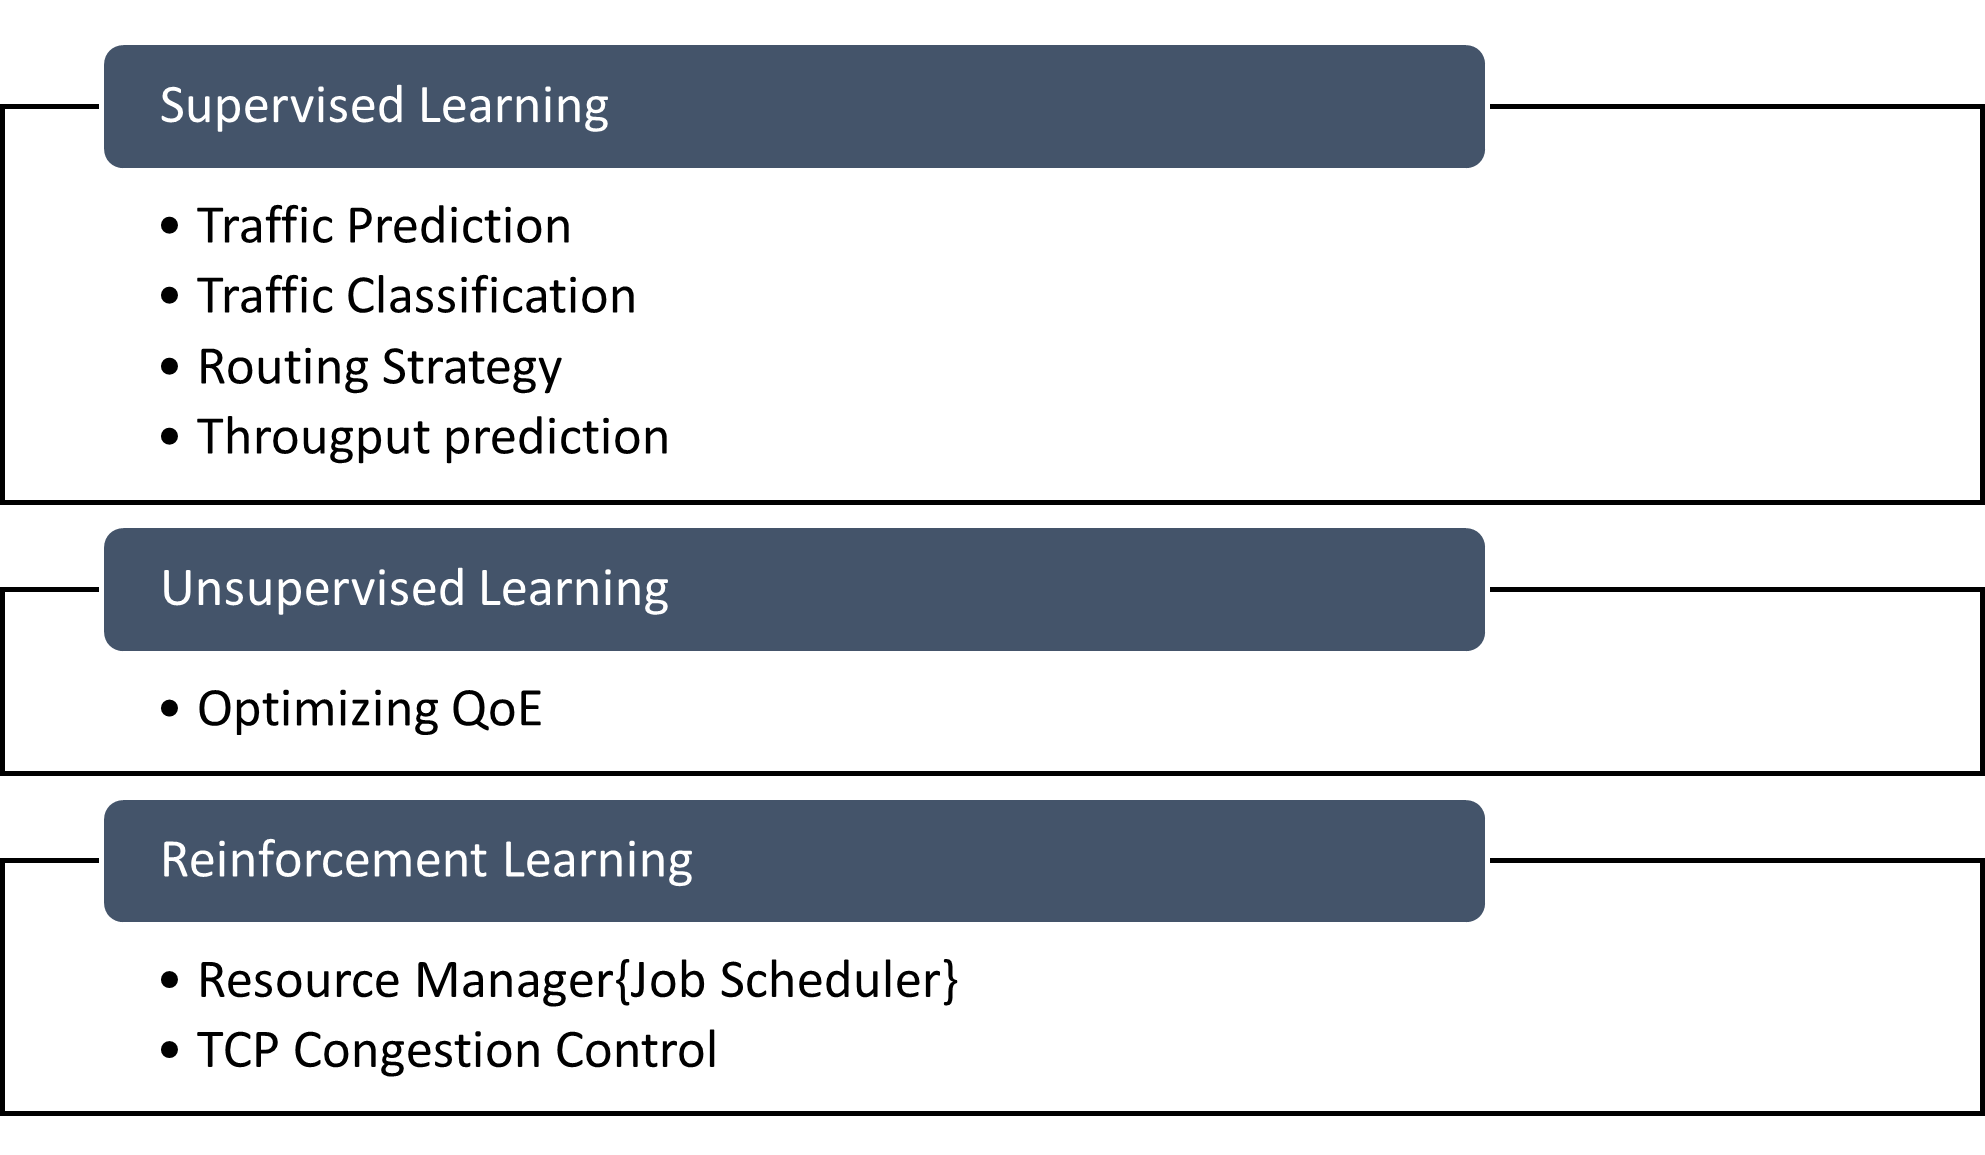
\includegraphics[width=.75\textwidth,height=.62\textheight]{RicercaMLNetworking.png}
    \end{figure}
\end{frame}

\begin{frame}
    \frametitle{MLN}
    \begin{figure}
        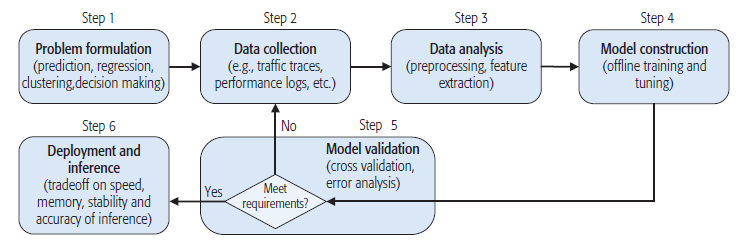
\includegraphics[width=.95\textwidth,height=.42\textheight]{WorkFlowNetworking.png}
    \end{figure}
    

\end{frame}
\subsection{Insider Threat Detection}
\begin{frame}
    \frametitle{Insider Threat Detection}
    \begin{figure}
        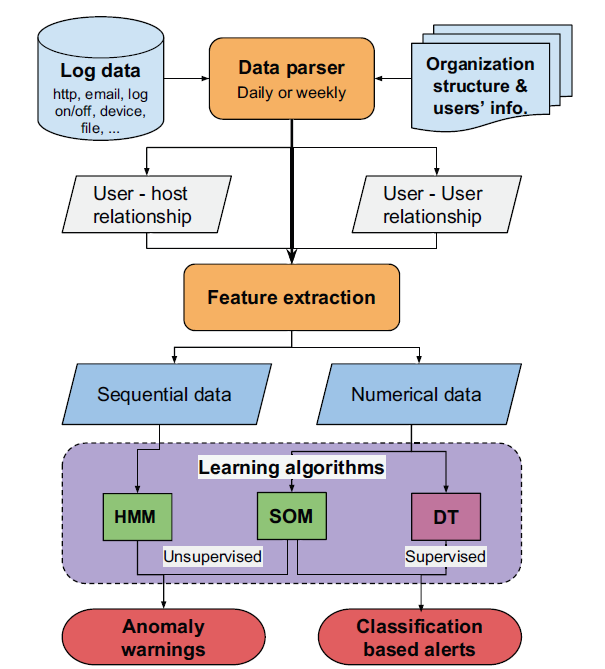
\includegraphics[width=.60\textwidth,height=.80\textheight]{workflowIntrusionThreat.png}
    \end{figure}
\end{frame}

\section{Analisi}

\begin{frame}
    \frametitle{Invariante di Processo}
    Analizzato i dversi casi di studio, abbiamo cercato di astrarre i problemi evidenziando un pattern generico di invariante.
    \begin{figure}[htbp]
        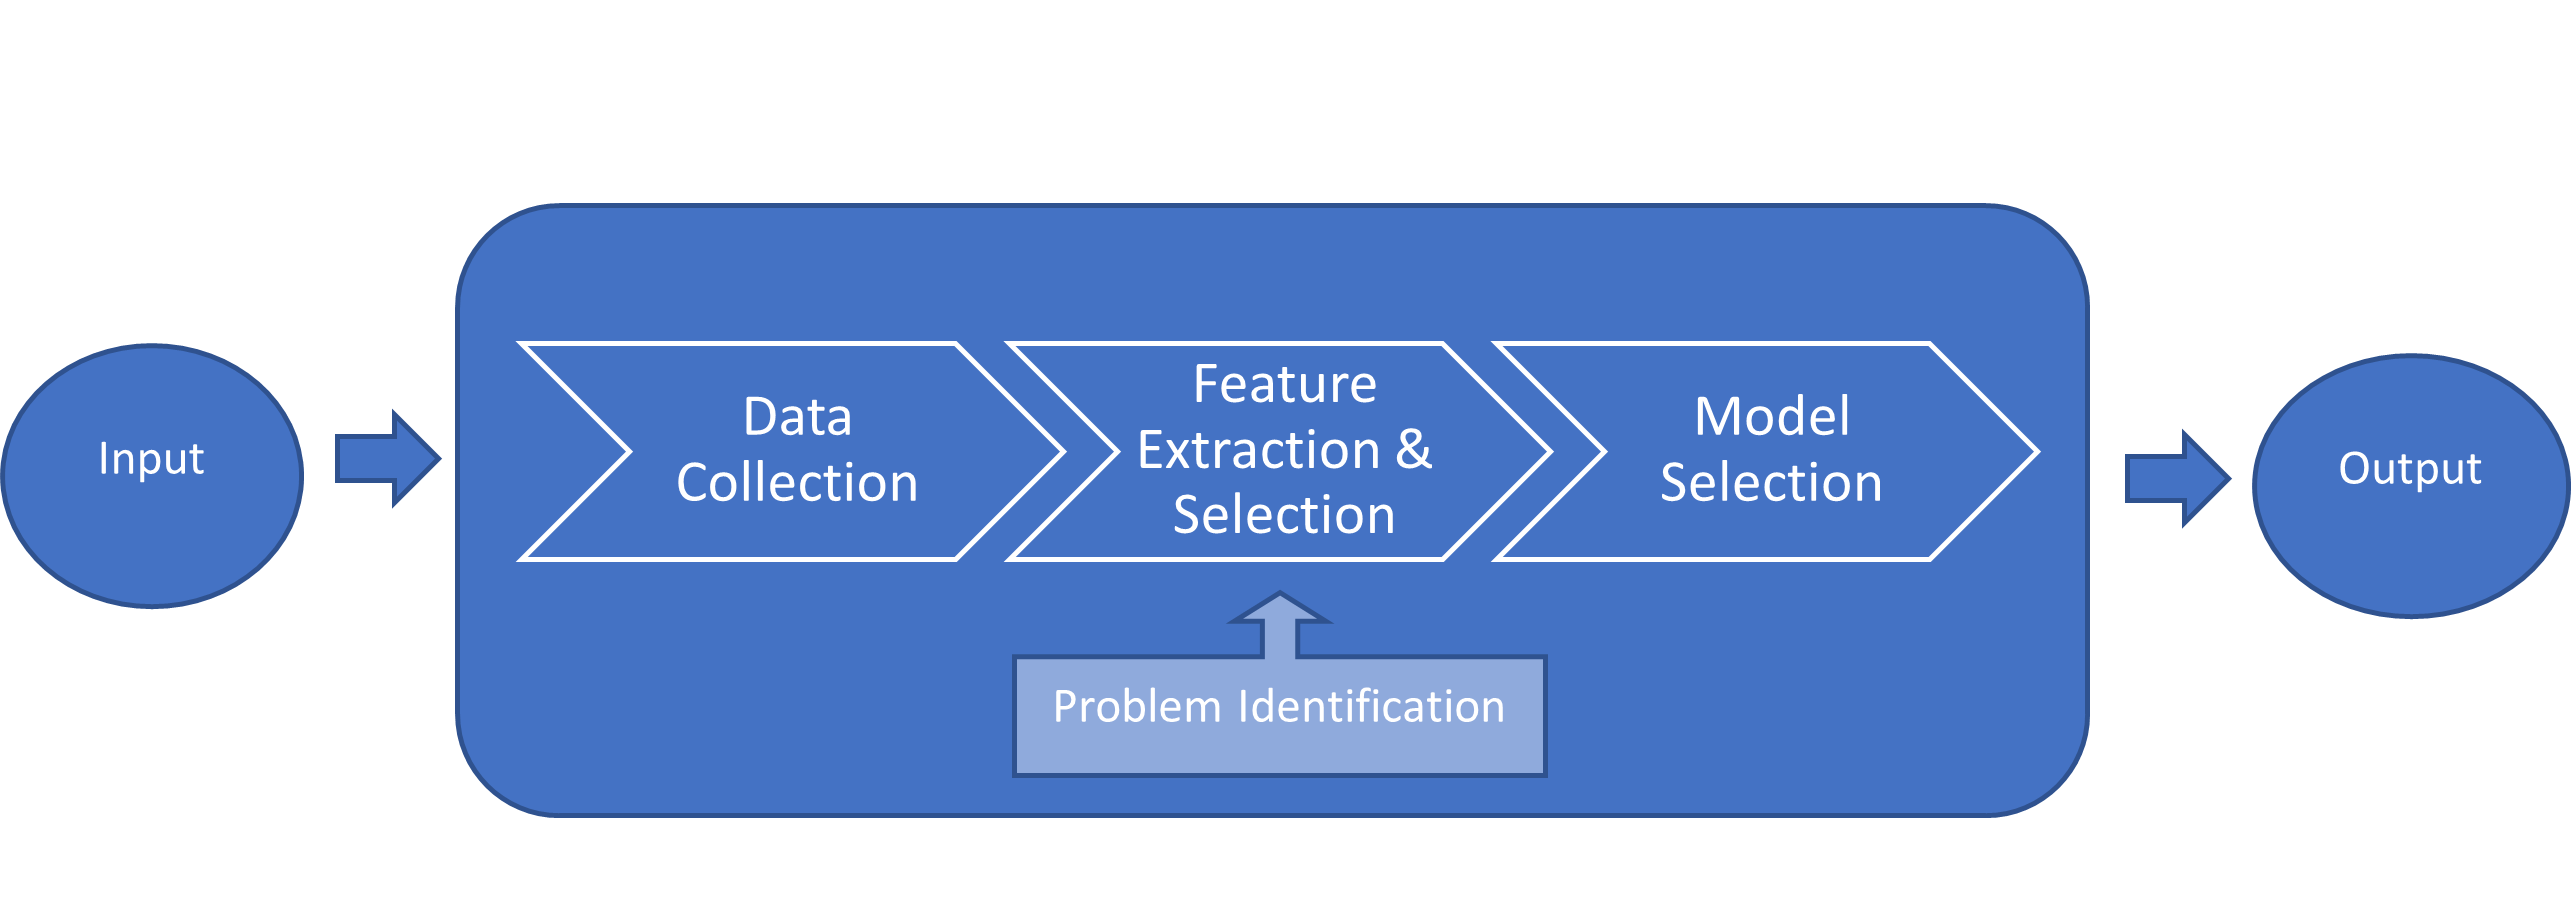
\includegraphics[width=0.9\textwidth]{Immagine3.png}
    \end{figure}
\end{frame}

\begin{frame}
    \frametitle{Raccolta Dati}
    La raccolta dati é fondamentale in ogni processo di apprendimento automatico.
    Viene diversificata a seconda del problema che andremo a trattare.
    Di solito i dati vengono suddivisi a seconda della \alert{metodologia di raccolta}.
\end{frame}

\begin{frame}
    \frametitle{Elaborazione del Modello}
    \begin{figure}[htbp]
        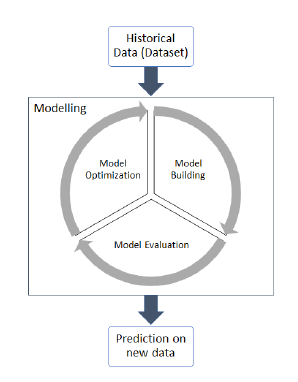
\includegraphics{MLProcess.png}
    \end{figure}
\end{frame}

\begin{frame}
    \frametitle{Risultato}
    In quest'ultima fase definiamo l'output desiderato:
    \begin{itemize}
        \item Classificazione
        \item Regressione 
        \item Clustering
    \end{itemize}
    \begin{figure}
        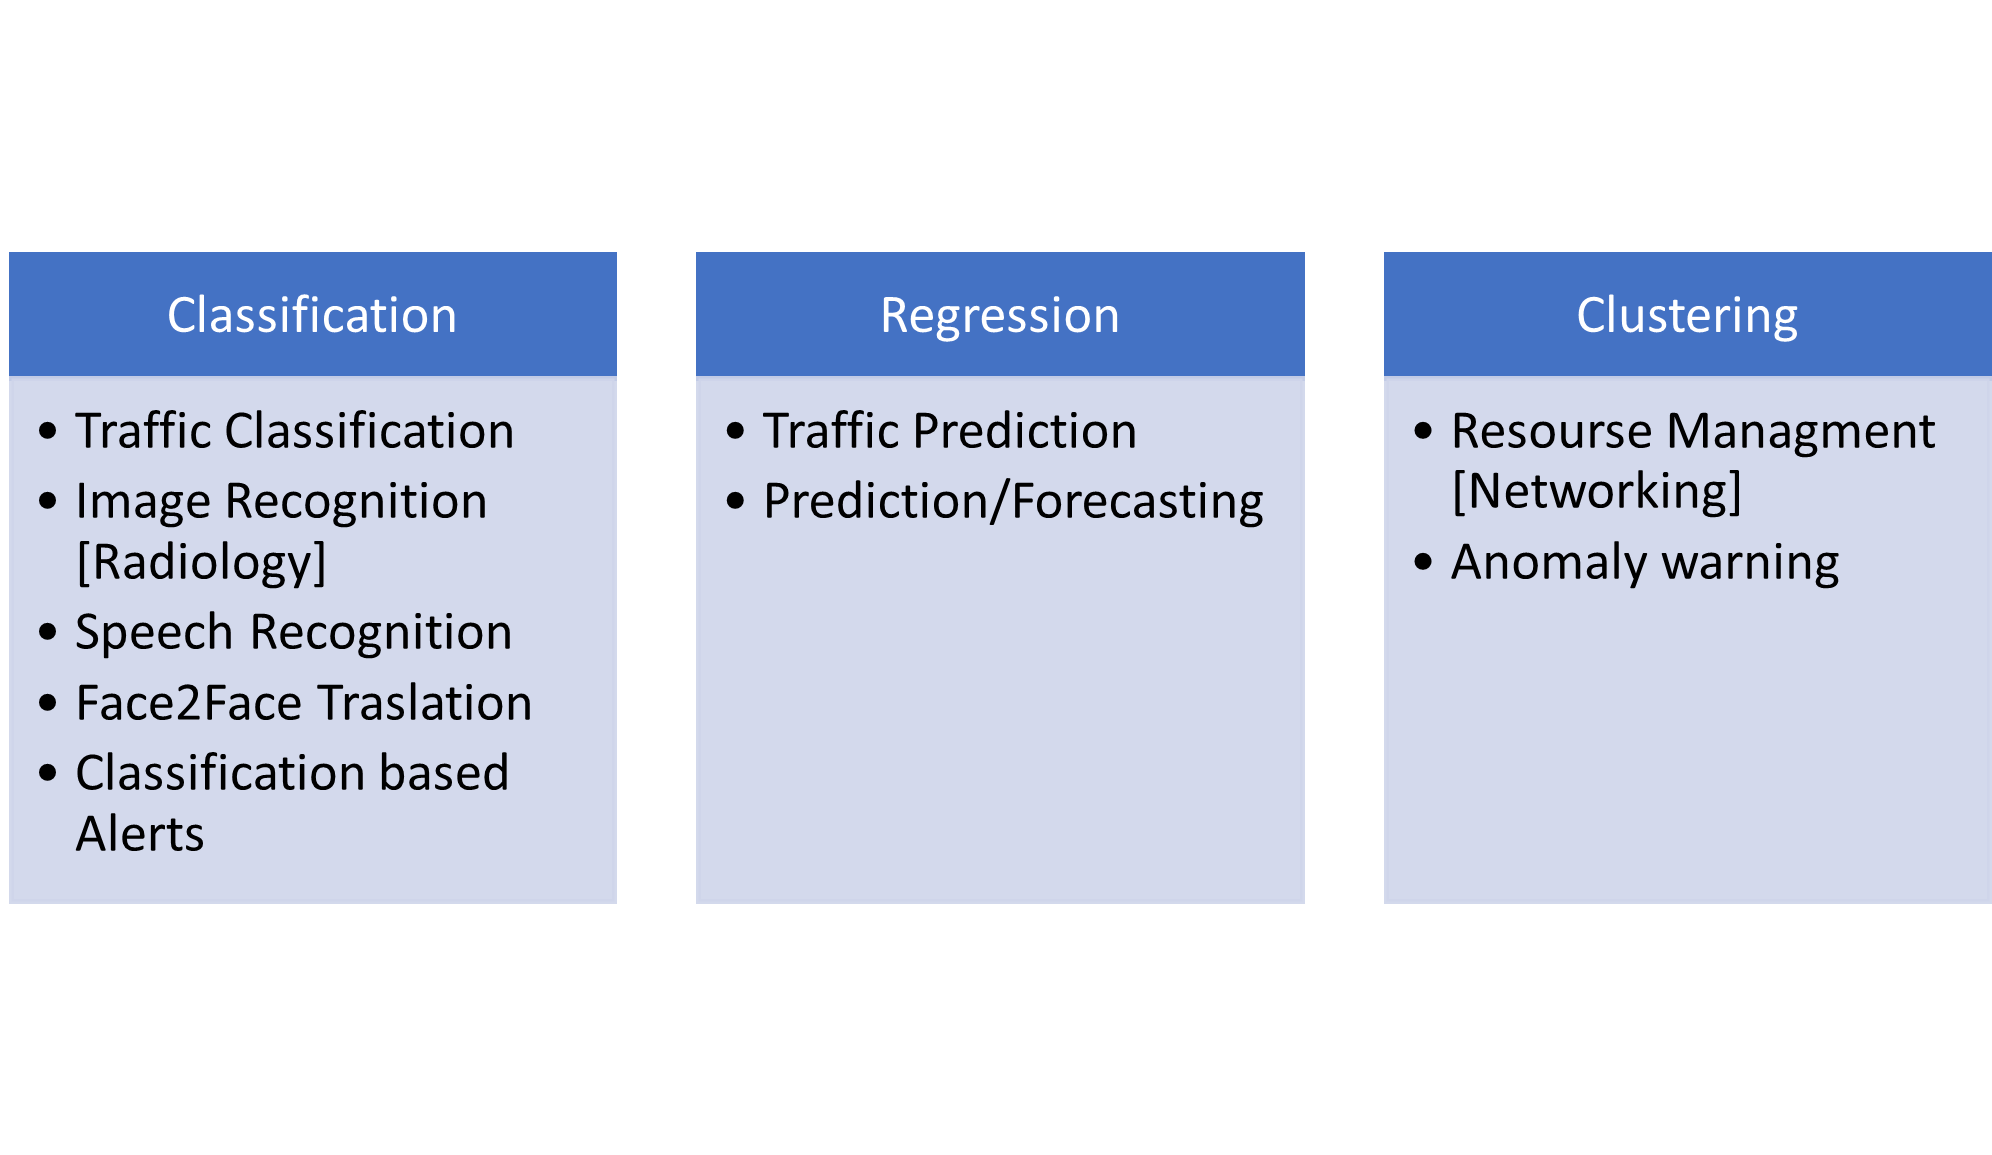
\includegraphics[width=0.9\textwidth , height=0.7\textheight]{categoryML.png}
    \end{figure}
\end{frame}
\section{Framework}

\begin{frame}    
        \frametitle{Framework}
        \newtheorem{fw}{Strumenti di Orchestrazione}

        \begin{fw}
            Questi strumenti che permettono l'orchestrazione di pipeline di Machine Learning  hanno l'obiettivo di semplificare il processo di gestione e automatizzare l'implementazione dei modelli di ML.
        \end{fw}
        Gli strumenti che andremo a mostrare di seguito sono tutti \textit{open-source}, e si focalizzano su 3 punti chiave:
        \begin{itemize}
            \item raccolta dati
            \item creazione e implementazione del modello
            \item distribuzione(permettendo inoltre la riproduzione ed il monitoraggio)
        \end{itemize}
\end{frame}
\begin{frame}
    \frametitle{ZenML}

    

\end{frame}

\begin{frame}
    \frametitle{Kedro}

    

\end{frame}

\begin{frame}
    \frametitle{Flyte}

    

\end{frame}

\begin{frame}
    \frametitle{MLRun}

    

\end{frame}
\end{document}
